\chapter{Medida del rendimiento}
\label{chap:medida_rendimiento}

\lettrine{L}{a} medida del rendimiento y el resultado de la misma es una parte fundamental en la evaluación y relevancia de un supercomputador, hasta el punto en el que se compite por ver cuales desarrollan un mejor resultado\footnote{\url{https://www.top500.org}}.

En este caso, si bien el rendimiento no es una prioridad, es conveniente realizar estas pruebas, especialmente para poder observar el impacto que tiene la red de comunicaciones entre los núcleos de una sola CPU, o entre múltiples CPUs y memorias. En resumen, medir la escalabilidad, que como se observa en \nameref{sec:comparacion_resultados} no es en absoluto espectacular.

\section{NAS Parallel Benchmarks}
Los \acrlong{npb} (\acrshort{npb})\footnote{\url{https://www.nas.nasa.gov/software/npb.html}} son una \textit{suite} de tests de cálculo numérico diseñados por la División de Supercomputación de la NASA para la medida del rendimiento de supercomputadores paralelos.

Estos benchmarks se dividen principalmente en ocho programas o \textit{kernels} (núcleos), teniendo otras adaptaciones para diferentes paradigmas de computación paralela, como puede ser de paralelización híbrida, computación desestructurada, o mallas de computación.

A su vez cada benchmark (\textit{kernel}) tiene múltiples clases, siendo estas \texttt{S}, \texttt{W}, \texttt{A}, \texttt{B}, \texttt{C}, \texttt{D}, \texttt{E}, y representando cada una un nivel de requerimientos superior, respectivamente. Específicamente, la las clases \texttt{A}, \texttt{B} y \texttt{C} suponen cuadruplicar el tamaño con respecto a la anterior, y las \texttt{D}, \texttt{E} y \texttt{F} (para los benchmarks que tienen estas clases disponibles), multiplican por 16 el tamaño del anterior.

En este caso se empleará la clase \texttt{C} para todos los benchmarks, excepto en \texttt{MG} que será clase \texttt{B}, y \texttt{FT}, que será clase \texttt{A}. Esta decisión para ambos benchmarks es así debido a limitaciones de memoria en las ejecuciones en un mismo nodo.

\subsection{Clases y procesos}
\label{ssec:clases_y_procesos}
Los benchmarks a ejecutar serán \texttt{LU}, \texttt{CG}, \texttt{FT}, \texttt{IS}, \texttt{MG} y \texttt{EP}, es decir, se excluyen \texttt{BT}, \texttt{SP} y \texttt{DT}. Esto es así debido a que los dos primeros requieren un número cuadrado perfecto de procesos, por lo que solo se podría ejecutar en 1, 4, 9, 16\dots\ procesos, y medir su rendimiento sería extraño debido a lo desbalanceado del mismo. En cuanto a \texttt{DT}, requiere una cantidad mínima de procesos en función de la clase del problema, procesos que para clase \texttt{A} y superior no son suficientes, por lo que se ha optado por descartarlo.

En concreto, los requerimientos para el número de procesos son los siguientes\footnote{Contenidos del fichero \texttt{README.install} en \texttt{NPB3.4-MPI}}:

\begin{lstlisting}
Different benchmark has different requirement for process count,
as listed below:

  BT, SP         - a square number of processes (1, 4, 9, ...)
  LU             - 2D (n1 * n2) process grid where n1/2 <= n2 <= n1
  CG, FT, IS, MG - a power-of-two number of processes (1, 2, 4, ...)
  EP, DT         - no special requirement
\end{lstlisting}

\subsection{Benchmarks}
\label{ssec:benchmarks}
Como se comenta en la subsección \ref{ssec:clases_y_procesos}, únicamente se ejecutarán algunos programas o kernels de medida del rendimiento por diversos motivos. Dentro de los que se ejecutan, y sabiendo que son todos de naturaleza numérica, es conveniente saber qué realiza (en mayor o menor medida, debido a la complejidad de los mismos) cada uno de ellos.

Los tamaños de problema en función de la clase se encuentran disponibles en \cite{npb_problem_sizes}, así como una explicación de los mismos en \cite{benchmarks1994technical}. 

\subsubsection{CG - Conjugate Gradient}
\label{sssec:benchmarks__cg}
El método del gradiente conjugado es un algoritmo para la resolución numérica de sistemas de ecuaciones lineales de matrices simétricas y definidas positivas. La explicación en profundidad del método se puede encontrar en \cite[2.2.3]{hestenes1952methods}, pero al quedar fuera del objetivo del trabajo, no se tratará en mayor profundidad, quedando como resumen que ``se trata de un método iterativo para resolución de sistemas de ecuaciones lineales'', siendo obvia su utilidad en aeronáutica, y de aquí su aparición en los \acrlong{npb}.

\subsubsection{EP - Embarrassingly Parallel}
\label{sssec:benchmarks__ep}
Este kernel ``embarazosamente parelelo'' tiene un nombre bastante descriptivo en cuanto a sus características, pero no en cuanto a su funcionamiento interno. Este programa sirve para estimar un límite superior al rendimiento en coma flotante, al que podrían aproximarse cargas de trabajo sin altos requerimientos de comunicación entre procesadores.

El kernel EP genera pares de números aleatorios siguiendo una distribución gaussiana, y los tabula en función de ciertos criterios que de nuevo, quedan fuera del alcance de este trabajo, pero que pueden ser consultados por usuarios más expertos en \cite[2.2.1]{benchmarks1994technical}. Este problema es típico de simulaciones estilo Monte Carlo y únicamente se requieren comunicaciones interprocesador al finalizar la ejecución para la realizacion de las (10) sumas del número de pares tabulados. 

\subsubsection{IS - Integer Sort}
\label{sssec:benchmarks__is}
Otro kernel con un nombre descriptivo, y es que hace lo que promete: Es un algoritmo paralelo de ordenación de números enteros. Como es evidente, este algoritmo no mide la capacidad en punto flotante del clúster, sino su capacidad de comparación de enteros, y especialmente la velocidad de su memoria debido a la cantidad de permutaciones que ocurren sobre la misma.

En un sistema de memoria compartida, las $N$ claves (es decir, cada número) se almacenan en un espacio de memoria contiguo. Sin embargo, en un espacio de memoria distribuida en $p$ secciones de memoria, se almacenan $N_{p}$ claves por espacio de memoria, siendo $N_{p} = N / p$.

Esta necesidad de ancho de banda a la memoria principal, así como de rápidas comunicaciones entre múltiples nodos se puede observar a la perfección en la sección \ref{ssec:comparacion_resultados__is}. Puede leerse con más detalle el funcionamiento del benchmark en \cite[2.2.5]{benchmarks1994technical}

\subsubsection{LU - Lower-Upper solver}
\label{sssec:benchmarks__lu}
La factorización LU es es un método de factorización de una matriz en dos matrices triangulares inferior y superior. Si ``factorización de matrices'' pudiera sonar extraño a algún lector, realmente no es nada esotérico: algunas matrices, al igual que algunos números enteros, pueden ser separadas en dos matrices, producto de las cuales se obtiene la matriz original.

Esta factorización se emplea en el análisis numérico para la resolución de sistemas de ecuaciones de forma más eficiente, por lo que, de nuevo, se puede apreciar la utilidad de este proceso en aeronáutica.

\begin{figure}[h!]
  \vspace*{0.5cm}
  \centering
  
    $\begin{pmatrix}
    a_{11} & a_{12} & a_{13}\\
    a_{21} & a_{22} & a_{23}\\
    a_{31} & a_{32} & a_{33}
    \end{pmatrix}
    =
    \begin{pmatrix}
    1      & 0      & 0\\
    l_{21} & 1      & 0\\
    l_{31} & l_{32} & 1
    \end{pmatrix}
    \begin{pmatrix}
    u_{11} & u_{12} & u_{13}\\
    0      & u_{22} & u_{23}\\
    0      & 0      & u_{33}
    \end{pmatrix}
    $

  \caption{Factorización LU para matrices 3x3}
  \label{fig:factorizacion_lu}
  %\vspace*{0.1cm}
\end{figure}

\subsubsection{FT - 3D FFT PDE (Fourier Transform)}
Este kernel resuelve numéricamente cierta ecuación en derivadas parciales mediante el uso de transformadas rápidas de Fourier tridimensionales directas (\acrshort{fft} o \acrlong{fft}) e inversas (I\acrshort{fft} o Inverse \acrshort{fft}). Se puede encontrar mayor detalle en esta rama avanzada de las matemáticas en \cite[2.2.4]{benchmarks1994technical}.

La \acrshort{fft} es una implementación eficiente de la transformada discreta de Fourier para computadores, de muy especial utilidad en el tratamiento digital de señales y la resolución de ecuaciones en derivadas parciales, siendo este último el uso que se le da en este benchmark. 

Las \acrshort{fft} en 3D son parte muy importante de aplicaciones en mecánica de fluidos, especialmente en simulaciones de torbellinos. Asimismo, la ejecución de estos algoritmos conlleva una importante comunicación entre procesos, lo cual tiene cierto impacto en las cifras de rendimiento, como se puede observar en \ref{ssec:comparacion_resultados__ft}.

\subsubsection{MG - MultiGrid}
Finalmente, el último benchmark que se ejecuta de esta suite es el multigrid. El proceso consiste en la realización de cuatro iteraciones del algoritmo multigrid de ciclo en V, que se emplean para la obtención de una aproximación a la solución $u$ de una ecuación de Poisson discreta, en una malla 256x256x256. Más información para lectores experimentados en este campo está disponible, de nuevo, en \cite[2.2.2]{benchmarks1994technical}.

Este método multigrid se emplea para la resolución de sistemas de ecuaciones diferenciales, y ha sido ampliamente utilizado para la resolución de otros sistemas de ecuaciones más complicados como las ecuaciones de Lamé o las Navier-Stokes. Ambas estas ecuaciones relacionadas con mecánica de fluidos, y por tanto y de nuevo, resultando sencillo visualizar la interconexión de esta carga de trabajo con aquellas empleadas en el campo de la aerodinámica.  

\subsection{Metodología}
La metodología es una muy importante parte en cualquier medida y análisis de la realidad, ya que permite filtrar y categorizar datos como más o menos fidedignos. En este caso la metodología a seguir ha sido moderadamente sencilla.

Se han realizado 5 ejecuciones de todos los problemas clase C, y 9 ejecuciones de los clase A o B. Esto es así, ya que a menor tiempo de ejecución, mayor probabilidad de obtener un dato atípico. Por suerte, y muy probablemente debido a la instalación mínima del sistema operativo, no ha habido variaciones significativas entre ejecuciones.

Los resultados de cada ejecución concreta de los benchmarks pueden encontrarse en el Apéndice \ref{chap:bench_values}.

\subsection{Prerrequisitos}
Para poder realizar las medidas de rendimiento, primero se necesitan tanto las herramientas de compilación como las de ejecución. Estas dependencias se deben satisfacer ejecutando en todos los nodos:

\begin{lstlisting}[language=bash]
# Se añade la opción --needed debido a que hay paquetes del metapaquete base-devel que ya están instalados, y no es necesario reinstalar.
# Tras ejecutar el comando se aceptan las opciones por defecto
pacman -S base-devel openmpi gcc-fortran wget --needed
\end{lstlisting}

\subsection{Instalación de los \acrshort{npb}}
A continuación se deben descargar, configurar, y compilar los \acrlong{npb} únicamente en el nodo maestro. Esto se realizará como \texttt{mpiuser} en la carpeta \texttt{/mpishared} de la siguiente forma:

\begin{lstlisting}[language=bash]
# Descarga de la última versión de NPB (3.4.2)
wget https://www.nas.nasa.gov/assets/npb/NPB3.4.2.tar.gz

# Descomprimir el archivo descargado
tar xzfv NPB3.4.2.tar.gz

# Y entrar en la versión de los NPB con MPI
cd /mpishared/NPB3.4.2/NPB3.4-MPI

# Copiar los archivos de configuración para la compilación
#  1- Para el archivo make.def se añaden un par de argumentos a los flags de compilación:
#   1.1- -fallow-argument-mismatch Esto permite que el código compile en las últimas versiones de gfortran
#   1.2- -march=native Optimiza para la arquitectura específica de rpi4
sed 's/^FFLAGS\s*=\s*-O3/FFLAGS  = -O3 -fallow-argument-mismatch -march=native/g' config/make.def.template | sed -e 's/^CFLAGS\s*=\s*-O3/CFLAGS  = -O3 -march=native/g' > config/make.def

#  2- Para el archivo suite.def se hace que todos los tests sean clase C menos FT, que por razones de memoria es clase A, y MG clase B, por los mismos motivos.
sed 's/S$/C/g' config/suite.def.template | sed -e 's/ft\s*C$/ft\tA/g' | sed -e 's/mg\s*C$/mg\tB/g' > config/suite.def

# Finalmente se compilan todos los tests con make suite (con todas las CPU en paralelo) $ TODO REMOVE CLOSING DOLLAR
make suite -j4
\end{lstlisting}

\subsection{Preparativos para la ejecución de los benchmarks}
Para la ejecución de los benchmarks de forma paralela se necesita algún método para coordinar la ejecución del programa en todos los nodos.

\begin{itemize}
    \item Para un solo nodo con múltiples núcleos es sencillo, ya que comparten memoria, usuarios y almacenamiento
    \item Para múltiples nodos sin embargo es algo más complejo. Como ya se menciona en las Subsecciones \ref{ssec:gen_ssh} y \ref{ssec:serv_nfs}, es necesario disponer de:
    \begin{itemize}
        \item Almacenamiento compartido en forma de NFS para alojar los ejecutables
        \item Autenticación y gestión común para el lanzamiento de los programas paralelos en forma de SSH con par de claves
    \end{itemize}
\end{itemize}

A MPI se le indica qué nodos deben ejecutar las tareas mediante un archivo de hosts, o \textit{hostsfile}\cite{mpi_hostfile_option}. Este fichero contiene las direcciones de los diferentes computadores que componen el clúster, así como el número de tareas que pueden ejecutar (habitualmente coincidente con su número de núcleos)

Así, se crea en \texttt{/mpishared} el fichero \texttt{hostfile} con los hostname de todos los nodos:

\begin{lstlisting}[language=bash]
rpi0 slots=4
rpi1 slots=4
rpi2 slots=4
rpi3 slots=4
rpi4 slots=4
rpi5 slots=4
rpi6 slots=4
rpi7 slots=4
\end{lstlisting}

\subsection{Ejecución de los benchmarks}
La ejecución de cada uno de los benchmarks se realizará mediante el siguiente comando \textbf{como usuario mpiuser}, en el que se debe especificar el número de procesos a crear, así como el hostfile. La sintaxis de este comando se comenta brevemente en \nameref{sssec:ejecucion_mpi}.\footnote{Se añade \texttt{--mca opal\_warn\_on\_missing\_libcuda 0} para evitar una advertencia que no interesa en la salida por pantalla}

\begin{lstlisting}[language=bash]
mpirun -np <NUM_PROCS> --hostfile /mpishared/hostfile --mca opal_warn_on_missing_libcuda 0 /mpishared/NPB3.4.2/NPB3.4-MPI/bin/<KERNEL>.<CLASS>.x
\end{lstlisting}

Como estos parámetros son fijos, es posible scriptear la ejecución de los benchmarks, así como la recolección de resultados, siempre y cuando solamente exista una clase por benchmark:

\begin{lstlisting}[language=bash]
#!/bin/sh

mkdir -p "results"

BENCHMARKS=( lu cg ft is mg ep )
MPIRUNFLAGS="--mca opal_warn_on_missing_libcuda 0"

for i in "${BENCHMARKS[@]}"
do
    for j in 1 2 4 8 16 32
    do
        mpirun -np $j --hostfile /mpishared/hostfile $MPIRUNFLAGS /mpishared/NPB3.4.2/NPB3.4-MPI/bin/${i}.*.x | tee -a results/$i.$j.run
    done
done
\end{lstlisting}

Ante diferentes números de procesos, \acrshort{mpi} elige la configuración más óptima, intentando mantener siempre las CPUs lo más cerca posible.

\section{Comparación de Resultados}
\label{sec:comparacion_resultados}
La comparación de resultados es precisamente el objetivo de los benchmarks. En este caso interesa medir la escalabilidad del clúster, y no compararlo contra otros. Esto es, medir la eficacia con la que, aumentando los recursos computacionales aumenta el rendimiento en la misma medida.

Se muestran a continuación los datos expresados en MOPS (\textbf{M}ega/\textbf{M}illion \textbf{O}perations \textbf{P}er \textbf{S}econd). En función de si estas operaciones son en punto flotante o no, también se podrán llamar \acrshort{mflops} (\textbf{M}ega/\textbf{M}illion \textbf{FL}oating point \textbf{O}perations \textbf{P}er \textbf{S}econd).

Esta métrica, MOPS, indica para cada benchmark el número de operaciones que realiza el kernel, que no el número de operaciones de la propia CPU. Por esta razón los resultados son muy diferentes y variados entre diferentes kernels. \cite[V. Performance Evaluation: B. NPB Kernels Performance on the Gigabit Ethernet cluster]{mallon2009npb}

Finalmente aclarar que en las gráficas se puede encontrar una línea vertical discontinua en los 4 núcleos. Esta línea señala la transición de ejecución en un solo computador (memoria compartida por 4 procesos) a ejecución en múltiples computadores, comunicados a través de Gigabit Ethernet (memoria distribuída en $N_{bloques}$ de 4 procesos, tal que $N_{bloques} = N_{procesos} / 4$). Además, debajo de dichas gráficas se encuentran dos medidores, siendo estos capturas de pantalla del \textit{Dashboard} de Clúpiter. La primera de ellas es para la ejecución en un solo nodo, y la segunda para ejecución en multinodo, siendo esta segunda una captura de un nodo al azar diferente al nodo maestro, ya que todos los nodos muestran un gráfico idéntico.

Si uno es perspicaz puede notar que el tráfico del nodo maestro es superior al del resto de nodos cuando el tráfico es muy reducido. Esto es así, porque es el nodo maestro el encargado de alojar la página web interactiva, y por tanto de recabar y enviar la información de monitorización de todos los nodos y mostrarla al usuario. Así, fijándose en alguna figura de un benchmark donde no haya intensivas comunicaciones (Fig. \ref{fig:mops__ep}), se puede comprobar que, si el nodo maestro tiene que recibir información de 7 nodos, y estos generan un tráfico de aproximadamente $60$ kbps (\ref{fig:mops_rev_mn__ep}), se puede ver fácilmente por qué en el nodo maestro (\ref{fig:mops_rev_sn__ep}) existe un tráfico de $416 \approx 420 = 60 \cdot 7$ kbps.

\subsection{CG}
\label{ssec:comparacion_resultados__cg}

Como puede apreciarse en la Figura \ref{fig:mops__cg}, el benchnmark CG es un benchmark mixto, en el que se realiza computación y comunicación de forma no diferenciada en el tiempo. Esto no parece ser un importante problema a la hora de entrar en modo de memoria distribuída, donde los MOPS por proceso no solo se estabilizan más o menos en la misma tendencia, sino que debido al dato atípicamente bajo para 4 procesadores en memoria compartida, el rendimiento mejora. Este valor atípicamente bajo podría deberse, como se va a ver posteriormente en múltiples ocasiones, al reducido ancho de banda de la memoria principal.

\begin{figure}[h!]
    \centering
    \begin{subfigure}[b]{0.495\textwidth}
        \begin{adjustbox}{width=\linewidth,height=0.8\linewidth}   
            \begin{tikzpicture}
                \begin{axis}[
                    xmin = 1, xmax = 32, xmode=log, log basis x=2, xticklabels={1,2,4,8,16,32}, xlabel=\#CPU,
                    ymin = 0, ylabel=MOPS total,
                    %width = \textwidth,
                    %height = 0.5\textwidth,
                    grid=both,
                ]
                \addplot[udcpink,smooth,very thick,mark=*] coordinates {
                    (1,115.37)
                    (2,158.44)
                    (4,112.03)
                    (8,319.65)
                    (16,565.98)
                    (32,1534.13)
                };

                \vasymptote {4};

                \legend{CG MOPS total};
                \end{axis}
            \end{tikzpicture}
        \end{adjustbox}
        % \caption
        \label{fig:mops_total__cg}
    \end{subfigure}
    \begin{subfigure}[b]{0.495\textwidth}
        \begin{adjustbox}{width=\linewidth,height=0.8\linewidth}   
            \begin{tikzpicture}
                \begin{axis}[
                    xmin = 1, xmax = 32, xmode=log, log basis x=2, xticklabels={1,2,4,8,16,32}, xlabel=\#CPU,
                    ymin = 0, ylabel=MOPS/proceso,
                    %width = \textwidth,
                    %height = 0.5\textwidth,
                    grid=both,
                ]

                \addplot[udcpink,smooth,very thick,mark=*] coordinates {
                    (1,115.37)
                    (2,79.22)
                    (4,28.01)
                    (8,39.96)
                    (16,35.37)
                    (32,47.94)
                };

                \vasymptote {4};

                \legend{CG MOPS/proceso};
                \end{axis}
            \end{tikzpicture}
        \end{adjustbox}
        %\caption
        \label{fig:mops_process__cg}
    \end{subfigure}

    \begin{subfigure}[c]{0.9\textwidth}
        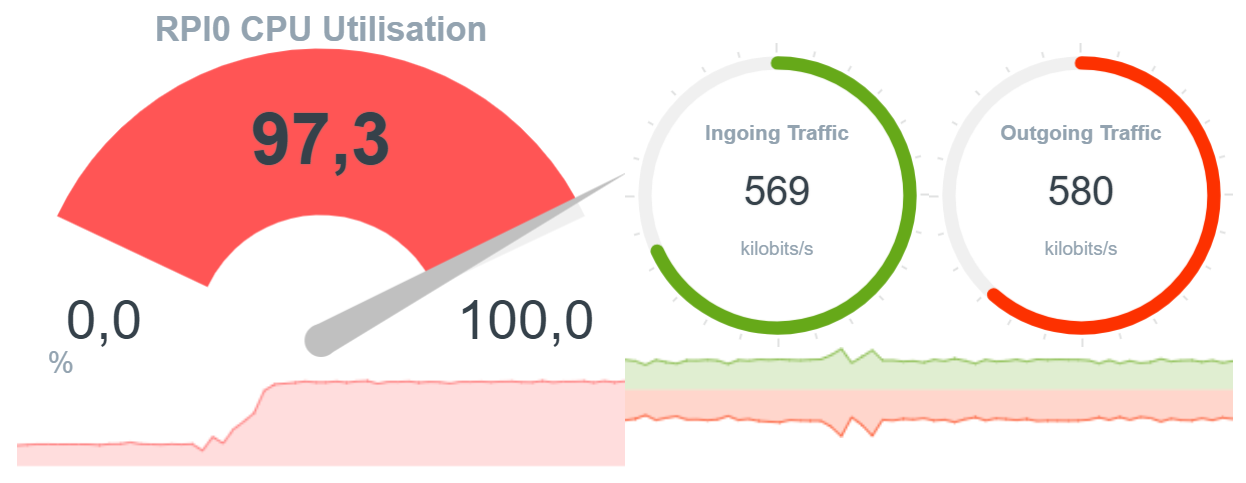
\includegraphics[width=\textwidth]{img/benchmark_rev/cg_rev_sn.png}
        \caption{Utilización de CPU para mononodo}
        \label{fig:mops_rev_sn__cg}
    \end{subfigure}

    \vspace{0.5cm}
    
    \begin{subfigure}[c]{0.9\textwidth}
        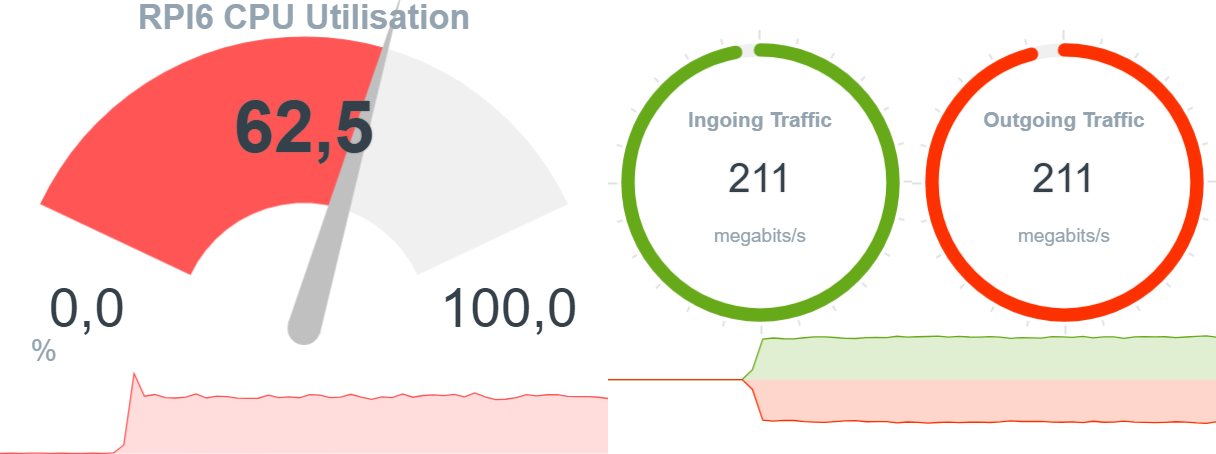
\includegraphics[width=\textwidth]{img/benchmark_rev/cg_rev_mn.png}
        \caption{Utilización de CPU y red para multinodo}
        \label{fig:mops_rev_mn__cg}
    \end{subfigure}
    \caption{Métricas de rendimiento, CPU y red para el kernel CG}
    \label{fig:mops__cg}
\end{figure}

\subsection{EP}
\label{ssec:comparacion_resultados__ep}
Por otro lado, como se puede ver en la Figura \ref{fig:mops__ep}, así como se comenta en \nameref{sssec:benchmarks__ep}, y en anteposición al benchmark discutido anteriormente, EP es un benchmark que realiza toda la computación de forma completamente independiente, y únicamente se comunica al final de la ejecución, siendo esta comunicación muy ligera, e indistinguible del tráfico habitual entre nodos (Fig. \ref{fig:mops_rev_mn__ep}). Además en este benchmark, hay de nuevo un valor atípicamente bajo para 4 procesadores, marcando una tendencia que, como se comenta anteriormente, probablemente sea debida al reducido ancho de banda del único chip de memoria DRAM en la \acrlong{rpi} 4B.

\begin{figure}[h!]
    \centering
    \begin{subfigure}[b]{0.495\textwidth}
        \begin{adjustbox}{width=\linewidth,height=0.8\linewidth}   
            \begin{tikzpicture}
                \begin{axis}[
                    xmin = 1, xmax = 32, xmode=log, log basis x=2, xticklabels={1,2,4,8,16,32}, xlabel=\#CPU,
                    ymin = 0, ylabel=MOPS total,
                    %width = \textwidth,
                    %height = 0.5\textwidth,
                    grid=both,
                ]
                \addplot[udcpink,smooth,very thick,mark=*] coordinates {
                    (1,31.91)
                    (2,62.84)
                    (4,112.45)
                    (8,236.25)
                    (16,446.06)
                    (32,868.45)
                };

                \vasymptote {4};

                \legend{EP MOPS total};
                \end{axis}
            \end{tikzpicture}
        \end{adjustbox}
        % \caption
        \label{fig:mops_total__ep}
    \end{subfigure}
    \begin{subfigure}[b]{0.495\textwidth}
        \begin{adjustbox}{width=\linewidth,height=0.8\linewidth}   
            \begin{tikzpicture}
                \begin{axis}[
                    xmin = 1, xmax = 32, xmode=log, log basis x=2, xticklabels={1,2,4,8,16,32}, xlabel=\#CPU,
                    ymin = 26, ylabel=MOPS/proceso,
                    %width = \textwidth,
                    %height = 0.5\textwidth,
                    grid=both,
                ]

                \addplot[udcpink,smooth,very thick,mark=*] coordinates {
                    (1,31.91)
                    (2,31.42)
                    (4,28.11)
                    (8,29.53)
                    (16,27.88)
                    (32,27.14)
                };

                \vasymptote {4};

                \legend{EP MOPS/proceso};
                \end{axis}
            \end{tikzpicture}
        \end{adjustbox}
        %\caption
        \label{fig:mops_process__ep}
    \end{subfigure}

    \begin{subfigure}[c]{0.9\textwidth}
        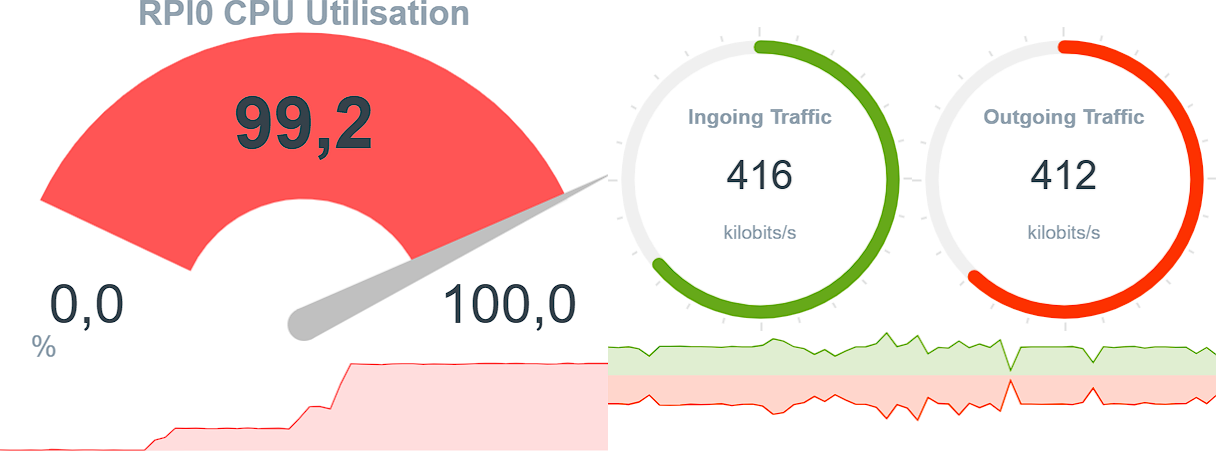
\includegraphics[width=\textwidth]{img/benchmark_rev/ep_rev_sn.png}
        \caption{Utilización de CPU para mononodo}
        \label{fig:mops_rev_sn__ep}
    \end{subfigure}

    \vspace{0.5cm}
    
    \begin{subfigure}[c]{0.9\textwidth}
        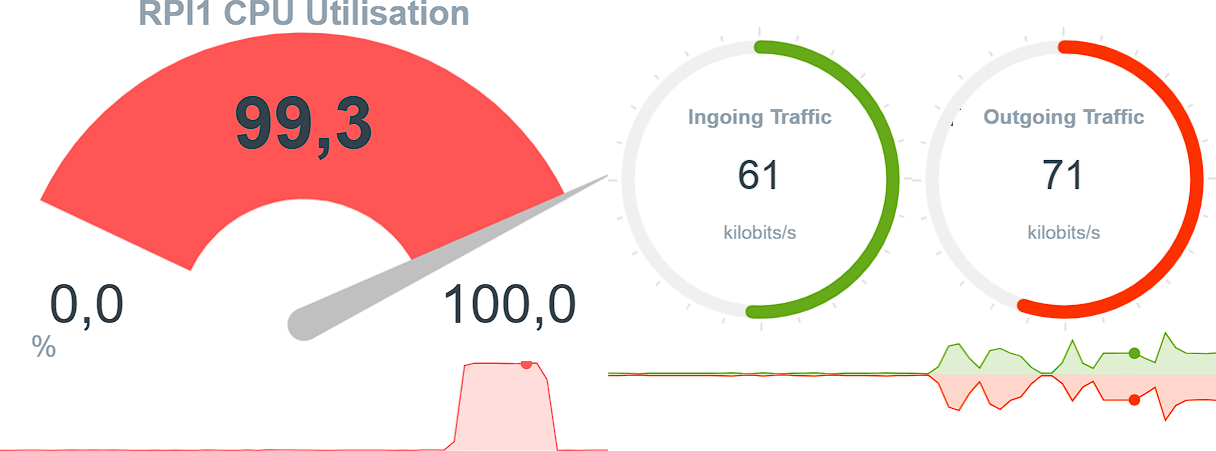
\includegraphics[width=\textwidth]{img/benchmark_rev/ep_rev_mn.png}
        \caption{Utilización de CPU y red para multinodo}
        \label{fig:mops_rev_mn__ep}
    \end{subfigure}
    \caption{Métricas de rendimiento, CPU y red para el kernel EP}
    \label{fig:mops__ep}
\end{figure}

\subsection{IS}
\label{ssec:comparacion_resultados__is}
El núcleo (kernel) IS es otro que realiza muy importantes movimientos de datos tanto de lectura como de escritura en memoria. Esto es un problema, como ya se discute previamente, debido al pequeño ancho de banda con la memoria principal. Combinado además con que la arquitectura \acrshort{arm} es del tipo \textit{load-store}, y las operaciones de red no están aceleradas por hardware, apunta a que el resultado probablemente no va a ser espectacular ni en mononodo, ni en multinodo. Esto puede confirmarse observando la Figura \ref{fig:mops__is}.

\begin{figure}[h!]
    \centering
    \begin{subfigure}[b]{0.495\textwidth}
        \begin{adjustbox}{width=\linewidth,height=0.8\linewidth}   
            \begin{tikzpicture}
                \begin{axis}[
                    xmin = 1, xmax = 32, xmode=log, log basis x=2, xticklabels={1,2,4,8,16,32}, xlabel=\#CPU,
                    ymin = 0, ylabel=MOPS total,
                    %width = \textwidth,
                    %height = 0.5\textwidth,
                    grid=both,
                ]
                \addplot[udcpink,smooth,very thick,mark=*] coordinates {
                    (1,38.29)
                    (2,60.75)
                    (4,78.42)
                    (8,54.77)
                    (16,67.20)
                    (32,92.70)
                };

                \vasymptote {4};

                \legend{IS MOPS total};
                \end{axis}
            \end{tikzpicture}
        \end{adjustbox}
        % \caption
        \label{fig:mops_total__is}
    \end{subfigure}
    \begin{subfigure}[b]{0.495\textwidth}
        \begin{adjustbox}{width=\linewidth,height=0.8\linewidth}   
            \begin{tikzpicture}
                \begin{axis}[
                    xmin = 1, xmax = 32, xmode=log, log basis x=2, xticklabels={1,2,4,8,16,32}, xlabel=\#CPU,
                    ymin = 0, ylabel=MOPS/proceso,
                    %width = \textwidth,
                    %height = 0.5\textwidth,
                    grid=both,
                ]

                \addplot[udcpink,smooth,very thick,mark=*] coordinates {
                    (1,38.29)
                    (2,30.37)
                    (4,19.60)
                    (8,6.85)
                    (16,4.20)
                    (32,2.90)
                };

                \vasymptote {4};

                \legend{IS MOPS/proceso};
                \end{axis}
            \end{tikzpicture}
        \end{adjustbox}
        %\caption
        \label{fig:mops_process__is}
    \end{subfigure}

    \begin{subfigure}[c]{0.9\textwidth}
        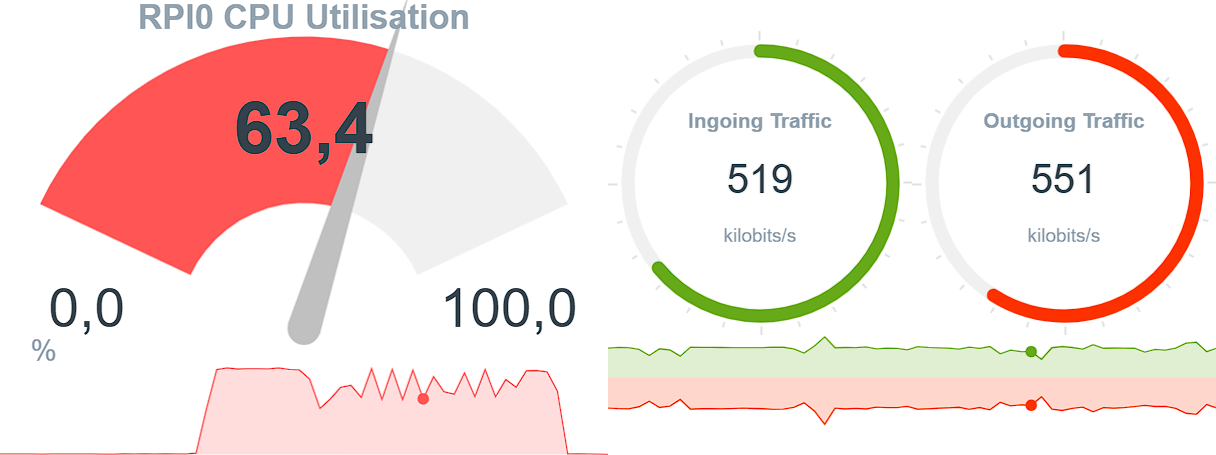
\includegraphics[width=\textwidth]{img/benchmark_rev/is_rev_sn.png}
        \caption{Utilización de CPU para mononodo}
        \label{fig:mops_rev_sn__is}
    \end{subfigure}

    \vspace{0.5cm}
    
    \begin{subfigure}[c]{0.9\textwidth}
        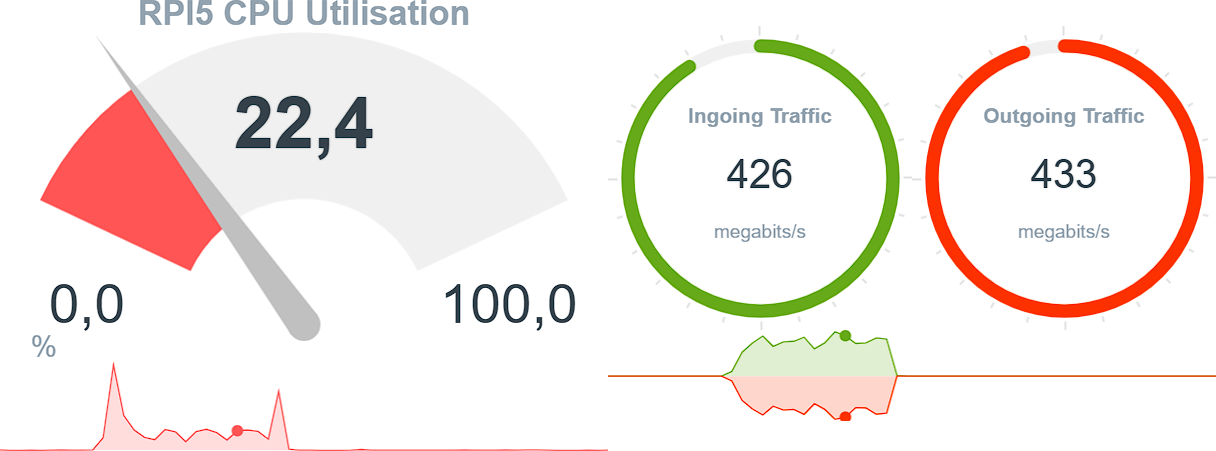
\includegraphics[width=\textwidth]{img/benchmark_rev/is_rev_mn.png}
        \caption{Utilización de CPU y red para multinodo}
        \label{fig:mops_rev_mn__is}
    \end{subfigure}
    \caption{Métricas de rendimiento, CPU y red para el kernel IS}
    \label{fig:mops__is}
\end{figure}

\subsection{LU}
\label{ssec:comparacion_resultados__lu}
De aquí en adelante vemos un escalado más normal (Fig. \ref{fig:mops__lu}), sin tantos datos atípicos, en donde se puede observar una caída de en torno al $60\textasciitilde70\%$ en MOPS por proceso al aumentar el número de procesos en el mismo nodo. Caída en picado que se vuelve más leve cuando se ejecuta en modo de memoria distribuída (multinodo). De nuevo, esta caída en picado es probablemente por la elevada demanda de ancho de banda a la memoria principal, que no puede ser satisfecha por un solo chip.

\begin{figure}[h!]
    \centering
    \begin{subfigure}[b]{0.495\textwidth}
        \begin{adjustbox}{width=\linewidth,height=0.8\linewidth}   
            \begin{tikzpicture}
                \begin{axis}[
                    xmin = 1, xmax = 32, xmode=log, log basis x=2, xticklabels={1,2,4,8,16,32}, xlabel=\#CPU,
                    ymin = 0, ylabel=MOPS total,
                    %width = \textwidth,
                    %height = 0.5\textwidth,
                    grid=both,
                ]
                \addplot[udcpink,smooth,very thick,mark=*] coordinates {
                    (1,1194.68)
                    (2,1654.34)
                    (4,1941.11)
                    (8,3689.97)
                    (16,7239.81)
                    (32,13674.22)
                };

                \vasymptote {4};

                \legend{LU MOPS total};
                \end{axis}
            \end{tikzpicture}
        \end{adjustbox}
        % \caption
        \label{fig:mops_total__lu}
    \end{subfigure}
    \begin{subfigure}[b]{0.495\textwidth}
        \begin{adjustbox}{width=\linewidth,height=0.8\linewidth}   
            \begin{tikzpicture}
                \begin{axis}[
                    xmin = 1, xmax = 32, xmode=log, log basis x=2, xticklabels={1,2,4,8,16,32}, xlabel=\#CPU,
                    ymin = 0, ylabel=MOPS/proceso,
                    %width = \textwidth,
                    %height = 0.5\textwidth,
                    grid=both,
                ]

                \addplot[udcpink,smooth,very thick,mark=*] coordinates {
                    (1,1194.68)
                    (2,827.17)
                    (4,485.28)
                    (8,461.25)
                    (16,452.49)
                    (32,427.32)
                };

                \vasymptote {4};

                \legend{LU MOPS/proceso};
                \end{axis}
            \end{tikzpicture}
        \end{adjustbox}
        %\caption
        \label{fig:mops_process__lu}
    \end{subfigure}

    \begin{subfigure}[c]{0.9\textwidth}
        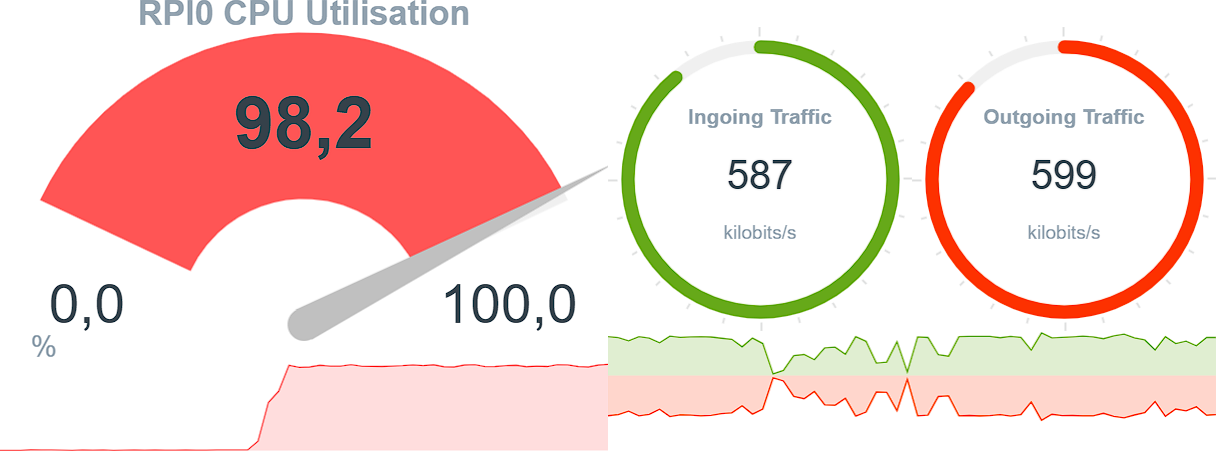
\includegraphics[width=\textwidth]{img/benchmark_rev/lu_rev_sn.png}
        \caption{Utilización de CPU para mononodo}
        \label{fig:mops_rev_sn__lu}
    \end{subfigure}

    \vspace{0.5cm}
    
    \begin{subfigure}[c]{0.9\textwidth}
        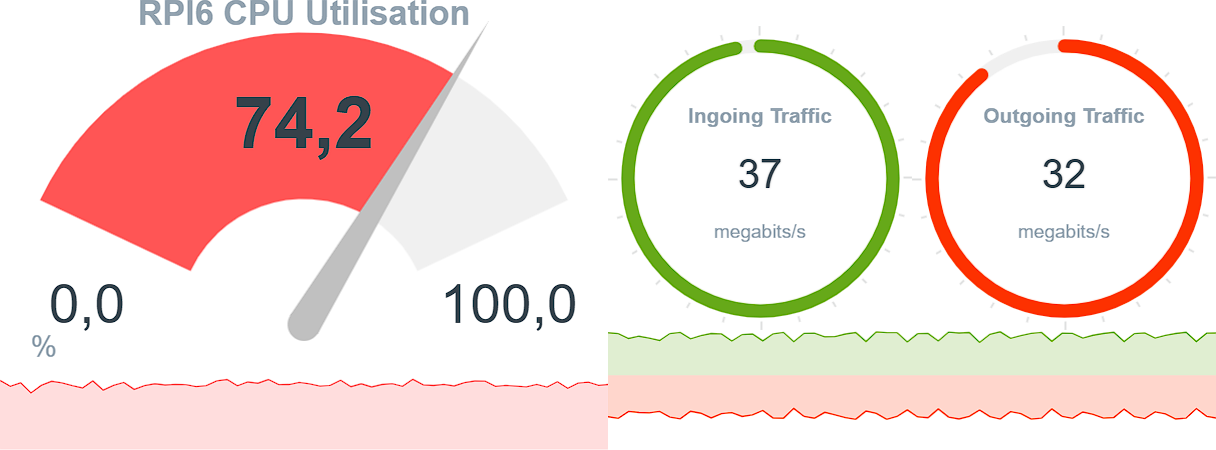
\includegraphics[width=\textwidth]{img/benchmark_rev/lu_rev_mn.png}
        \caption{Utilización de CPU y red para multinodo}
        \label{fig:mops_rev_mn__lu}
    \end{subfigure}
    \caption{Métricas de rendimiento, CPU y red para el kernel LU}
    \label{fig:mops__lu}
\end{figure}

\subsection{FT}
\label{ssec:comparacion_resultados__ft}
En este benchmark de resolución de ecuaciones en derivadas parciales mediante transformadas de Fourier tridimensionales se sigue la misma tendencia que en el kernel discutido previamente. Es interesante destacar que este benchmark, a pesar de ser intensivo en comunicaciones, éstas no se dan simultáneamente con el cómputo, sino que se alternan con el mismo, (Fig. \ref{fig:mops_rev_mn__ft}). Detalles del rendimiento para cada configuración de CPUs se encuentran en la Figura \ref{fig:mops__ft}.

\begin{figure}[h!]
    \centering
    \begin{subfigure}[b]{0.495\textwidth}
        \begin{adjustbox}{width=\linewidth,height=0.8\linewidth}   
            \begin{tikzpicture}
                \begin{axis}[
                    xmin = 1, xmax = 32, xmode=log, log basis x=2, xticklabels={1,2,4,8,16,32}, xlabel=\#CPU,
                    ymin = 0, ylabel=MOPS total,
                    %width = \textwidth,
                    %height = 0.5\textwidth,
                    grid=both,
                ]
                \addplot[udcpink,smooth,very thick,mark=*] coordinates {
                    (1,602.08)
                    (2,804.61)
                    (4,888.52)
                    (8,1069.91)
                    (16,1582.68)
                    (32,2584.08)
                };

                \vasymptote {4};

                \legend{FT MOPS total};
                \end{axis}
            \end{tikzpicture}
        \end{adjustbox}
        % \caption
        \label{fig:mops_total__ft}
    \end{subfigure}
    \begin{subfigure}[b]{0.495\textwidth}
        \begin{adjustbox}{width=\linewidth,height=0.8\linewidth}   
            \begin{tikzpicture}
                \begin{axis}[
                    xmin = 1, xmax = 32, xmode=log, log basis x=2, xticklabels={1,2,4,8,16,32}, xlabel=\#CPU,
                    ymin = 0, ylabel=MOPS/proceso,
                    %width = \textwidth,
                    %height = 0.5\textwidth,
                    grid=both,
                ]

                \addplot[udcpink,smooth,very thick,mark=*] coordinates {
                    (1,602.08)
                    (2,402.31)
                    (4,222.13)
                    (8,133.74)
                    (16,98.92)
                    (32,80.75)
                };

                \vasymptote {4};

                \legend{FT MOPS/proceso};
                \end{axis}
            \end{tikzpicture}
        \end{adjustbox}
        %\caption
        \label{fig:mops_process__ft}
    \end{subfigure}

    \begin{subfigure}[c]{0.9\textwidth}
        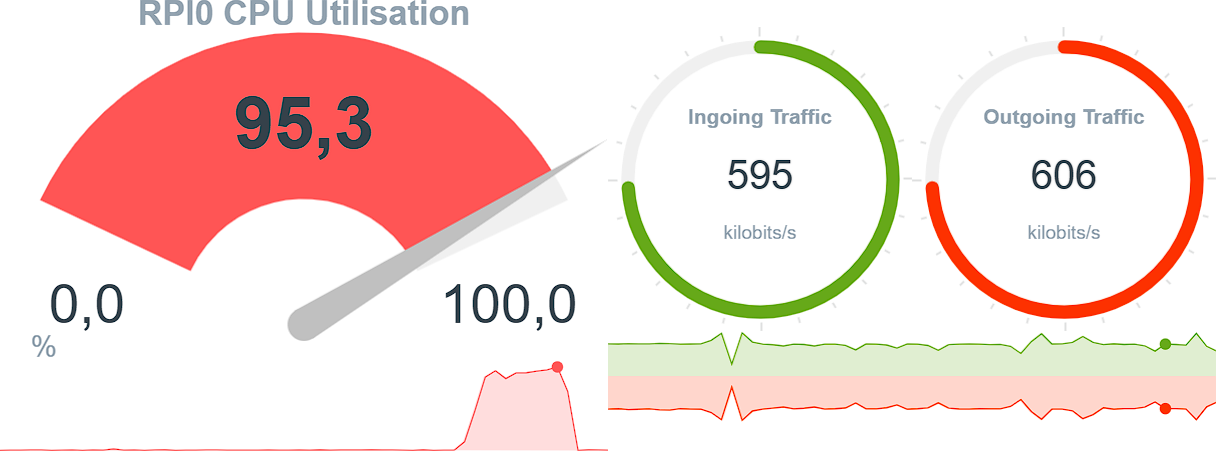
\includegraphics[width=\textwidth]{img/benchmark_rev/ft_rev_sn.png}
        \caption{Utilización de CPU para mononodo (Clase A)}
        \label{fig:mops_rev_sn__ft}
    \end{subfigure}

    \vspace{0.5cm}
    
    \begin{subfigure}[c]{0.9\textwidth}
        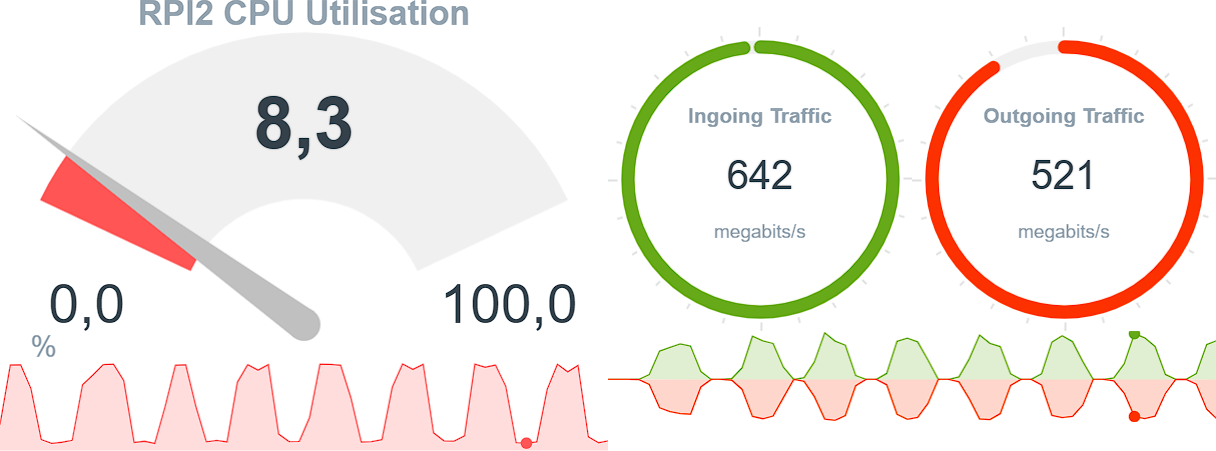
\includegraphics[width=\textwidth]{img/benchmark_rev/ft_rev_mn.png}
        \caption{Utilización de CPU y red para multinodo (Clase C)}
        \label{fig:mops_rev_mn__ft}
    \end{subfigure}
    \caption{Métricas de rendimiento, CPU y red para el kernel FT}
    \label{fig:mops__ft}
\end{figure}

\subsection{MG}
\label{ssec:comparacion_resultados__mg}
Por último se expone el rendimiento del benchmark Multigrid (\ref{fig:mops__mg}), que por las características de su algoritmo, realiza un importante uso de las comunicaciones interprocesador. En este kernel, el uso de RAM es muy intensivo, por lo que en un mismo nodo, al doblar el número de CPUs en uso, los MOPS por procesador se reducen casi a la mitad, obteniendo casi el mismo rendimiento, lo cual resulta bastante decepcionante.

\begin{figure}[h!]
    \centering
    \begin{subfigure}[b]{0.495\textwidth}
        \begin{adjustbox}{width=\linewidth,height=0.8\linewidth}   
            \begin{tikzpicture}
                \begin{axis}[
                    xmin = 1, xmax = 32, xmode=log, log basis x=2, xticklabels={1,2,4,8,16,32}, xlabel=\#CPU,
                    ymin = 0, ylabel=MOPS total,
                    %width = \textwidth,
                    %height = 0.5\textwidth,
                    grid=both,
                ]
                \addplot[udcpink,smooth,very thick,mark=*] coordinates {
                    (1,609.39)
                    (2,699.88)
                    (4,771.88)
                    (8,1462.09)
                    (16,2532.57)
                    (32,4499.23)
                };

                \vasymptote {4};

                \legend{MG MOPS total};
                \end{axis}
            \end{tikzpicture}
        \end{adjustbox}
        % \caption
        \label{fig:mops_total__mg}
    \end{subfigure}
    \begin{subfigure}[b]{0.495\textwidth}
        \begin{adjustbox}{width=\linewidth,height=0.8\linewidth}   
            \begin{tikzpicture}
                \begin{axis}[
                    xmin = 1, xmax = 32, xmode=log, log basis x=2, xticklabels={1,2,4,8,16,32}, xlabel=\#CPU,
                    ymin = 0, ylabel=MOPS/proceso,
                    %width = \textwidth,
                    %height = 0.5\textwidth,
                    grid=both,
                ]

                \addplot[udcpink,smooth,very thick,mark=*] coordinates {
                    (1,609.39)
                    (2,349.94)
                    (4,192.97)
                    (8,182.76)
                    (16,158.29)
                    (32,140.60)
                };

                \vasymptote {4};

                \legend{MG MOPS/proceso};
                \end{axis}
            \end{tikzpicture}
        \end{adjustbox}
        %\caption
        \label{fig:mops_process__mg}
    \end{subfigure}

    \begin{subfigure}[c]{0.9\textwidth}
        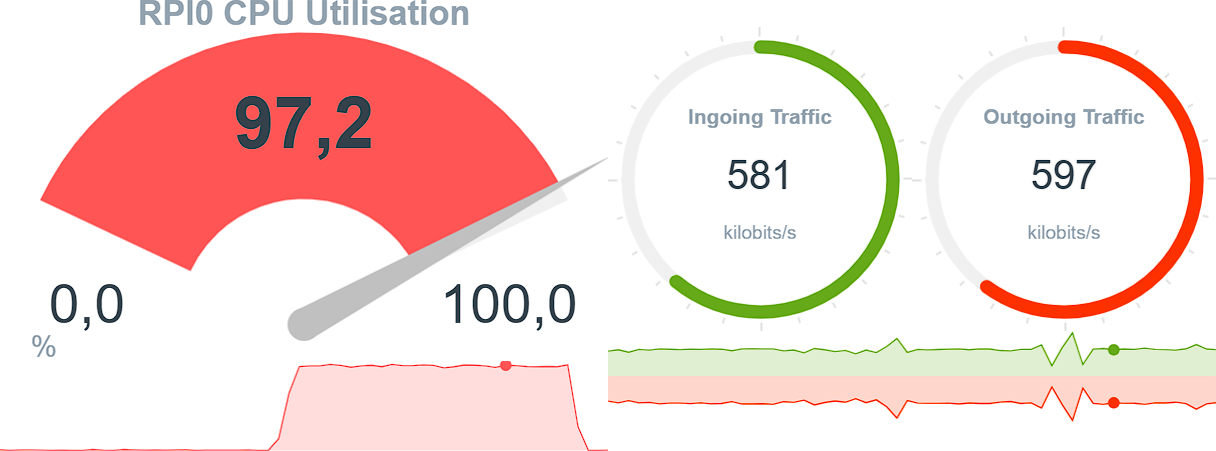
\includegraphics[width=\textwidth]{img/benchmark_rev/mg_rev_sn.png}
        \caption{Utilización de CPU para mononodo (Clase B)}
        \label{fig:mops_rev_sn__mg}
    \end{subfigure}

    \vspace{0.5cm}
    
    \begin{subfigure}[c]{0.9\textwidth}
        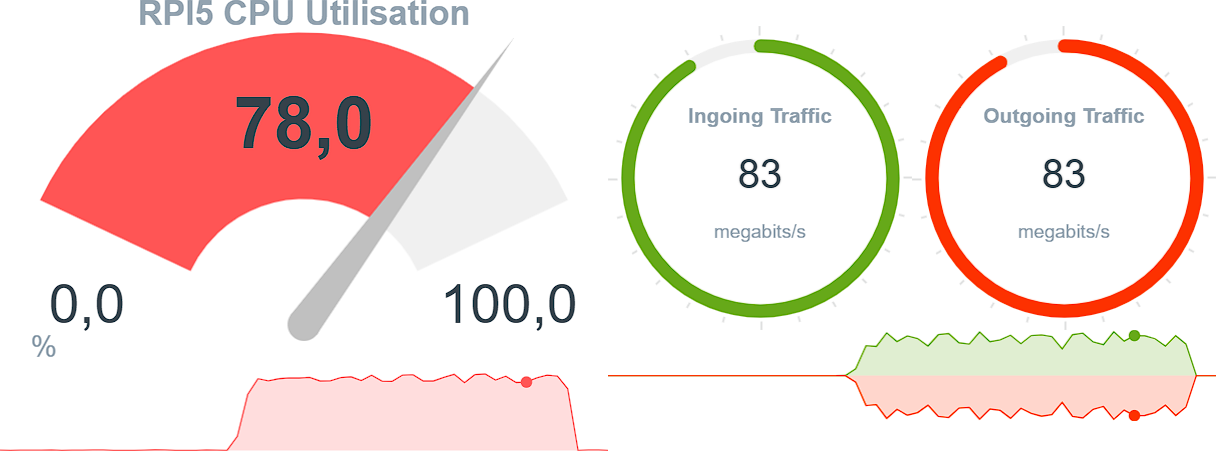
\includegraphics[width=\textwidth]{img/benchmark_rev/mg_rev_mn.png}
        \caption{Utilización de CPU y red para multinodo (Clase C)}
        \label{fig:mops_rev_mn__mg}
    \end{subfigure}
    \caption{Métricas de rendimiento, CPU y red para el kernel MG}
    \label{fig:mops__mg}
\end{figure}


